\documentclass[tikz,border=6pt]{standalone}
\usepackage{tikz}
\usetikzlibrary{arrows.meta,positioning,fit,calc}

\definecolor{inputgreen}{RGB}{235,241,219}
\definecolor{refyellow}{RGB}{255,247,213}
\definecolor{modelblue}{RGB}{229,239,255}
\definecolor{outpurple}{RGB}{239,232,250}
\definecolor{border}{RGB}{126,112,64}
\definecolor{arrowblue}{RGB}{57,119,190}

\tikzset{
  box/.style={draw=border, rounded corners=5pt, line width=0.8pt,
    align=center, inner sep=6pt, font=\sffamily\small},
  title/.style={font=\sffamily\bfseries\normalsize},
  item/.style={draw=border!75, rounded corners=3pt, fill=white,
    align=center, inner sep=3.5pt, font=\sffamily\scriptsize},
  flow/.style={-{Latex[length=2.2mm]}, line width=0.9pt, draw=arrowblue},
  note/.style={font=\sffamily\scriptsize\itshape, align=center}
}

\begin{document}
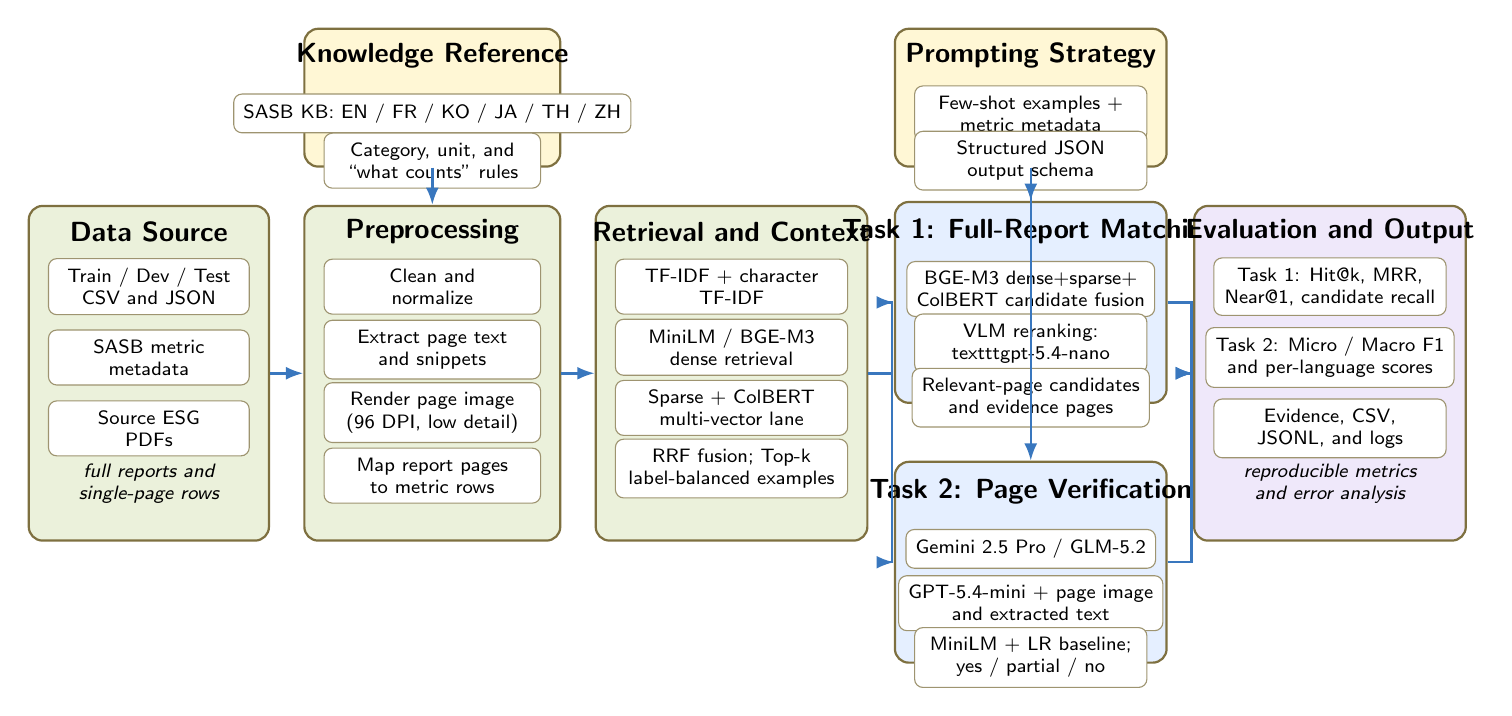
\begin{tikzpicture}[x=1cm,y=1cm]

% Main input and preprocessing stages
\node[box, fill=inputgreen, minimum width=3.05cm, minimum height=4.25cm] (data) at (1.65,2.65) {};
\node[title] at (1.65,4.45) {Data Source};
\node[item, minimum width=2.55cm] at (1.65,3.75) {Train / Dev / Test\\CSV and JSON};
\node[item, minimum width=2.55cm] at (1.65,2.85) {SASB metric\\metadata};
\node[item, minimum width=2.55cm] at (1.65,1.95) {Source ESG\\PDFs};
\node[note] at (1.65,1.25) {full reports and\\single-page rows};

\node[box, fill=inputgreen, minimum width=3.25cm, minimum height=4.25cm] (prep) at (5.25,2.65) {};
\node[title] at (5.25,4.45) {Preprocessing};
\node[item, minimum width=2.75cm] at (5.25,3.75) {Clean and\\normalize};
\node[item, minimum width=2.75cm] at (5.25,2.95) {Extract page text\\and snippets};
\node[item, minimum width=2.75cm] at (5.25,2.15) {Render page image\\(96 DPI, low detail)};
\node[item, minimum width=2.75cm] at (5.25,1.35) {Map report pages\\to metric rows};

% Knowledge reference above preprocessing
\node[box, fill=refyellow, minimum width=3.25cm, minimum height=1.75cm] (kb) at (5.25,6.15) {};
\node[title] at (5.25,6.68) {Knowledge Reference};
\node[item, minimum width=2.75cm] at (5.25,5.95) {SASB KB: EN / FR / KO / JA / TH / ZH};
\node[item, minimum width=2.75cm] at (5.25,5.35) {Category, unit, and\\``what counts'' rules};

% Retrieval/context stage
\node[box, fill=inputgreen, minimum width=3.45cm, minimum height=4.25cm] (retr) at (9.05,2.65) {};
\node[title] at (9.05,4.45) {Retrieval and Context};
\node[item, minimum width=2.95cm] at (9.05,3.75) {TF-IDF + character\\TF-IDF};
\node[item, minimum width=2.95cm] at (9.05,2.98) {MiniLM / BGE-M3\\dense retrieval};
\node[item, minimum width=2.95cm] at (9.05,2.21) {Sparse + ColBERT\\multi-vector lane};
\node[item, minimum width=2.95cm] at (9.05,1.44) {RRF fusion; Top-k\\label-balanced examples};

% Prompting strategy
\node[box, fill=refyellow, minimum width=3.45cm, minimum height=1.75cm] (prompt) at (12.85,6.15) {};
\node[title] at (12.85,6.68) {Prompting Strategy};
\node[item, minimum width=2.95cm] at (12.85,5.95) {Few-shot examples +\\metric metadata};
\node[item, minimum width=2.95cm] at (12.85,5.35) {Structured JSON\\output schema};

% Task 1 branch
\node[box, fill=modelblue, minimum width=3.45cm, minimum height=2.55cm] (task1) at (12.85,3.55) {};
\node[title] at (12.85,4.45) {Task 1: Full-Report Matching};
\node[item, minimum width=2.95cm] at (12.85,3.72) {BGE-M3 dense+sparse+\\ColBERT candidate fusion};
\node[item, minimum width=2.95cm] at (12.85,3.03) {VLM reranking: \\texttt{gpt-5.4-nano}};
\node[item, minimum width=2.95cm] at (12.85,2.34) {Relevant-page candidates\\and evidence pages};

% Task 2 branch
\node[box, fill=modelblue, minimum width=3.45cm, minimum height=2.55cm] (task2) at (12.85,0.25) {};
\node[title] at (12.85,1.15) {Task 2: Page Verification};
\node[item, minimum width=2.95cm] at (12.85,0.42) {Gemini 2.5 Pro / GLM-5.2};
\node[item, minimum width=2.95cm] at (12.85,-0.27) {GPT-5.4-mini + page image\\and extracted text};
\node[item, minimum width=2.95cm] at (12.85,-0.96) {MiniLM + LR baseline;\\yes / partial / no};

% Output stage
\node[box, fill=outpurple, minimum width=3.45cm, minimum height=4.25cm] (out) at (16.65,2.65) {};
\node[title] at (16.65,4.45) {Evaluation and Output};
\node[item, minimum width=2.95cm] at (16.65,3.75) {Task 1: Hit@k, MRR,\\Near@1, candidate recall};
\node[item, minimum width=2.95cm] at (16.65,2.85) {Task 2: Micro / Macro F1\\and per-language scores};
\node[item, minimum width=2.95cm] at (16.65,1.95) {Evidence, CSV,\\JSONL, and logs};
\node[note] at (16.65,1.25) {reproducible metrics\\and error analysis};

% Flow arrows
\draw[flow] (data.east) -- (prep.west);
\draw[flow] (kb.south) -- (prep.north);
\draw[flow] (prep.east) -- (retr.west);
\draw[flow] (retr.east) -- ++(0.30,0) |- (task1.west);
\draw[flow] (retr.east) -- ++(0.30,0) |- (task2.west);
\draw[flow] (prompt.south) -- (task1.north);
\draw[flow] (prompt.south) -- ++(0,-0.20) -| (task2.north);
\draw[flow] (task1.east) -- ++(0.30,0) |- (out.west);
\draw[flow] (task2.east) -- ++(0.30,0) |- (out.west);

\end{tikzpicture}
\end{document}
